\section{Data Reduction and Calibration}
\label{891_1:sec:data_reduction}

\subsection{Image processing and spectral extraction}

Basic reduction (overscan correction, bias/dark subtraction) were done
with IRAF's CCDPROC package. Cosmic rays were cleaned with the CRUTIL
package. Spectral extraction, wavelength calibration, and flux
calibration were done with the HYDRA package. The multiple fiber sizes
in \GP required modifications to the standard DOHYDRA procedure for
flat-field generation, sky-subtraction, and flux calibration. A
detailed walkthrough and discussion of these modifications can be
found at \url{www.astro.wisc.edu/~eigenbrot/GradPak}; we summarize the
important points below.

\subsubsection{Wavelength Calibration}
\label{891_1:sec:wavecal}

Uncertainties in the wavelength solution in the blue
($<$\val{4500}{\AA}) are the dominant source of uncertainty in
determining the line-of-sight doppler shift of the observed
spectra. As shown in Paper II, these velocities are important for
determining the line-of-sight depth of our spectroscopic observations,
which requires velocity precision better than the spectral resolution
of our data.
%% {\bf [QUESTION: for the purpose of velocities, why not
%%     just use the wavelengths longward of 4000? I think that would have
%%     been the right thing to do, but the broader point is that for
%%     doing chi$^2$ analysis down to H\&K we need wave calibration
%%     better than the spectral resolution. This is a point we echo in
%%     the last section on the instrumental dispersion so important to
%%     point it out here too: we need accurate first and second
%%     moments.]} 
The reason for the wavelength calibration uncertainty
at short wavelengths is the combined dearth of strong spectral
features in the CuAr arc-lamp and the sensitivity fall-off in the
fibers, spectrograph optics, grating and CCD. The number of good
spectral lines that can be fit from the available arc-lamps between
\val{4130}{\AA} and \val{7300}{\AA} is 33.

To characterize the uncertainties in the wavelength calibration, we
measure the centers of Solar Ca H\&K absorption (from zodiacal or
atmospheric scattering) and three HgI emission lines (atmospheric
scattering from terrestrial sources, e.g., Tucson) in our data before
sky subtraction. In all of our data exposures the foreground (zodiacal
plus atmospheric) signal dominated over the flux from NGC 891 to the
point where discrimination between Solar Ca H\&K and Ca H\&K in NGC
891 was not necessary.

For each night of observation all wavelength-calibrated object frames
are combined to improve S/N (especially relevant for measurements of
absorption lines) before line centroids are measured with IRAF's
FITPROFS routine. For each line measured the average offset from the
known center across all \GP fibers is taken as an indication of the
accuracy of the wavelength solution at that particular wavelength. The
standard deviation of the measured centers across all \GP fibers is a
measure of the precision of the wavelength solution at a particular
wavelength.

\begin{figure}
  \centering
  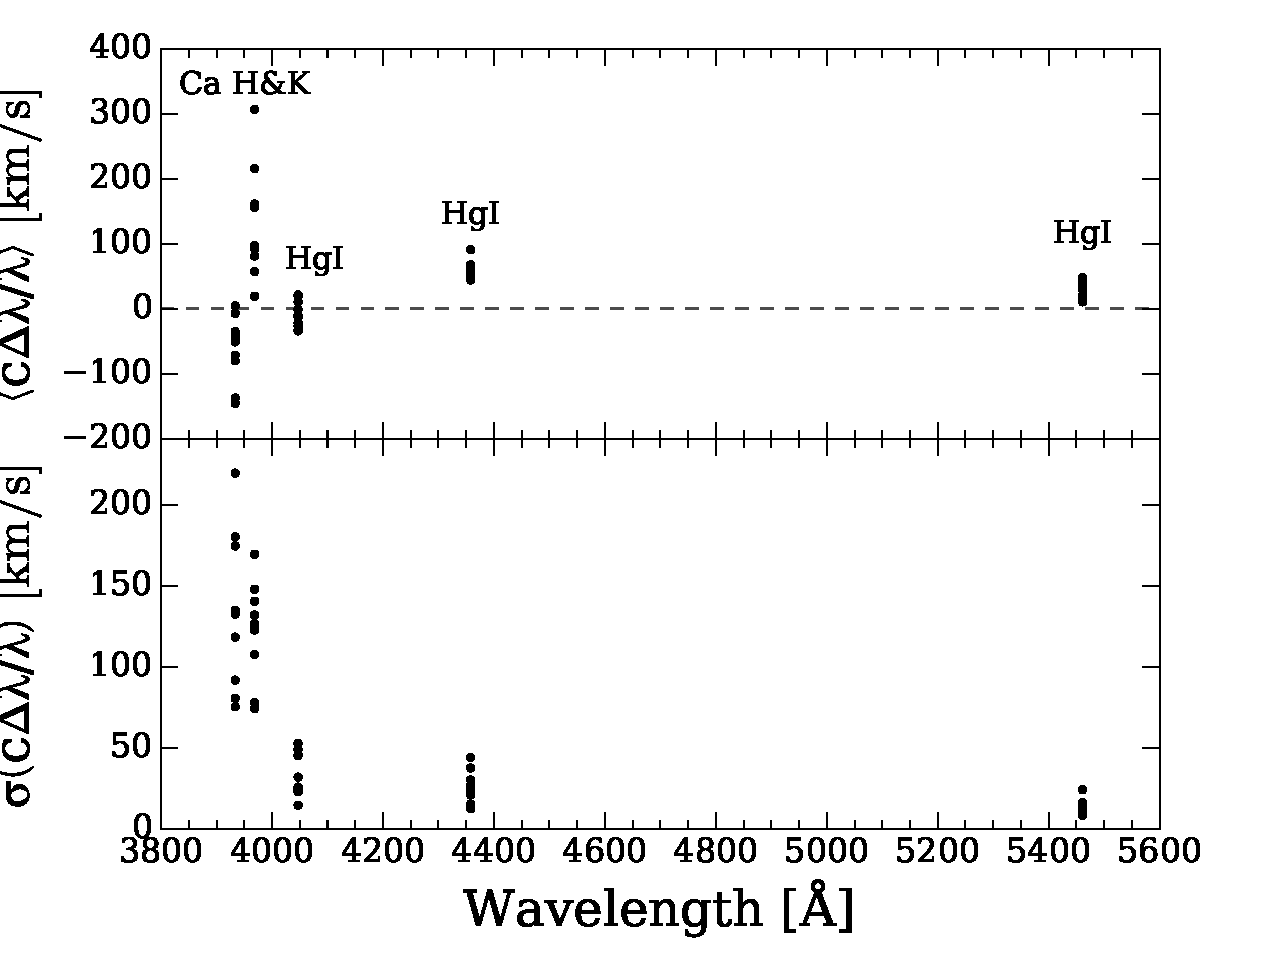
\includegraphics[width=\columnwidth]{891_1/figs/Wave_Err_comb.pdf}
  \caption[Accuracy and precision of wavelength
  calibration]{\label{891_1:fig:wave_err}\fixspacing Estimated accuracy and
    precision of the wavelength solution in the blue region of the
    spectrum based on measurements of known foreground features (HgI
    emission at 4047, 4358 and 5461 \AA\ from terrestrial light
    pollution, and Solar Fraunhofer H\&K lines from Ca) in our sky
    spectra.  Each point corresponds to a measurement of a line from
    an individual night of NGC 891 observations. \emph{top:} The mean
    offset in km $^{-1}$ between measured line centers and the known
    values, averaged over all \GP fibers. \emph{bottom:} The standard
    deviation of the measured line centers in km s$^{-1}$, computed
    across all \GP fibers.}
\end{figure}

Accordingly, Figure \ref{891_1:fig:wave_err} shows the estimated accuracy
and precision for each of the 10 nights of NGC 891 observations.  At
wavelengths $>\val{\asim 4000}{\AA}$ our wavelength solution is both
accurate and precise to within \val{\asim 50}{km/s}. Below
\val{4000}{\AA} (where the wavelength solution is determined via
extrapolation of the CuAr lamp line data) we measure a systematic
offset of \val{\asim 120}{km/s} with a comparable value for the random
error. We therefore report an upper limit on the uncertainty in our
wavelength solution to be \val{120}{km/s} at \val{4000}{\AA}, while
noting that for most wavelengths this is an overestimation.  The RMS
uncertainty reported by the wavelength fitting routine is \val{\asim
  90}{km/s}, which is likely a more accurate estimate of the
uncertainty for the wavelength region covered by arc lines
(\val{4130}{\AA}$<\lambda <$ \val{7300}{\AA}).  Even in the worst case
we are able to calibrate wavelengths to a higher precision than the
spectral resolution (see \S\ref{891_1:sec:GPak_dispersion}), which varies
from 180 to \val{570}{km/s} at \val{4000}{\AA} (depending on fiber
size). Thus, accurate measurements of velocity based on $\chi^2$
fitting of absorption lines (as done in Paper II) is possible with our
data.


%% The maximum offset from the true values give us an
%% upper limit on the uncertainty in our wavelength solution. Using this
%% method we find an upper limit of \val{\asim 100}{km/s} at
%% \val{4000}{\AA}, which is consistent with the value of \val{\asim
%%   90}{km/s} based on the RMS of the wavelength solution fit. {\bf
%%   [TODO: Let me get this straight: we are not using these features to
%%     improve the calibration, but just as a cross-check?]}

\begin{figure}
  \centering
  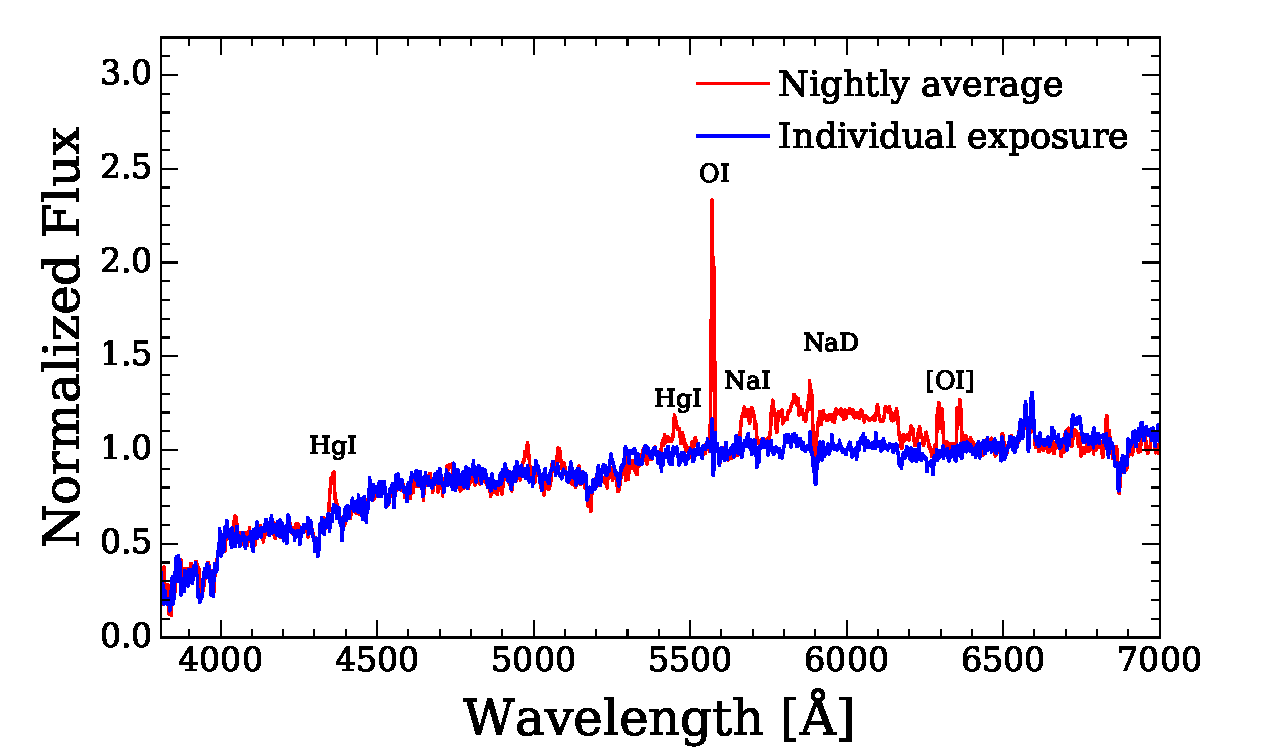
\includegraphics[width=\columnwidth]{891_1/figs/skysub_comp.pdf}
  \caption[Sky subtraction example]{\label{891_1:fig:skysub_comp}\fixspacing Example of large
    sky-subtraction residuals from November 21st, 2014. The red
    spectrum shows fiber 80 after sky subtraction using a sky spectrum
    that is the average across the whole night. The blue spectrum
    shows the same fiber using after sky subtraction using only the
    sky fibers from the same exposure. The large residuals around
    \val{6000}{\AA} (a broad high-pressure sodium feature) have been
    eliminated along with a number of strong, narrow emission lines.}
\end{figure}

\subsubsection{Flat Fields}
\label{891_1:sec:flats}

The combination of spectrograph setup and the multiple fiber sizes in
\GP required two different dome flat exposure times: a short exposure
(\val{1}{s}) to avoid saturating the largest fibers, and a long
exposure (\val{4}{s}) to get adequate signal in the smallest fibers.
%% Repeat
%  For this reason we took one set of \val{4}{s} dome flats to produce
% enough signal in the smallest fibers (while saturating the largest
% fibers) and one set of \val{1}{s} dome flats to avoid saturating the
% largest fibers (while getting almost no signal in the smallest
% fibers).
Both sets of dome flat exposures were run through CCDPROC, combined,
and had their apertures extracted independently by DOHYDRA.  The
so-called ``extraction'' produces a one-dimensional data vector
(spectrum) for each fiber. In both cases the extraction used fiber
traces computed from the \val{1}{s} flat for all data because we found
that saturated large fibers in the \val{4}{s} flats introduced errors
in the extraction process while the low signal in small fibers at
\val{1}{s} was still adequate for tracing purposes. In practice,
traces using the \val{4}{s} or \val{1}{s} are very similar, as
confirmed with the intermediate-size fibers that have good signal
without being saturated. This is expected given the fact that the two
exposure sets were taken right after each other over a short period of
time.

Once the two flats had their apertures extracted, the resulting
spectra were scaled to the same exposure time and stitched together
into a ``master'' flat where the 1.87'' and 2.81'' fibers were taken
from the \val{4}{s} flat and the 3.75'', 4.69'', and 5.62'' fibers
were taken from the \val{1}{s} flat. This master flat was used in all
subsequent reduction of the on-sky data.

During the exercise of establishing this pipeline we discovered a lag
in the shutter time that affects exposures shorter than \val{\asim
  7}{s}. The WIYN Bench Spectrograph CCD has a linear slide shutter
that has opening and closing times that are not equal. Because the
shutter moves along the wavelength dimension of the CCD the effect of
this inequality is to add an artificial spectral signature. The
magnitude of this signature varies with exposure time, with the
largest deviation measured as $\asim 20\%$ at \val{1}{s}. We removed
this spectral mismatch between the \val{1}{s} and \val{4}{s} flats by
normalizing all fibers in the \val{4}{s} flat to the mean spectrum of
the \val{1}{s} flat. While this method still introduces the shutter
spectrum present in the \val{4}{s} flat this spectrum is constant
across all fibers and is thus removed during flux calibration.

\subsubsection{Sky Subtraction}
\label{891_1:sec:skysub}

Each fiber size in \GP has 4 dedicated sky fibers, as illustrated in
Figure \ref{891_1:fig:GradPak}.  Sky subtraction was performed on a
fiber-size basis using different beam numbers for each fiber size in
HYDRA's SKYSUB routine.  Since there are multiple sky fibers rejection
of contaminated sky fibers was possible, as indeed was required (see
Figure \ref{891_1:fig:pointings} for P6, P4, P1).

The data from the night of November 21st, 2014 (P1) showed strong
variation in sky intensity across the course of the night. This
variation did not subtract well when using a sky spectrum averaged
across the whole night. In particular, the region between atmospheric
NaI emission at \val{5684}{\AA} and the broad high-pressure sodium
feature around \val{5900}{\AA} often left strong residuals when using
a nightly average for the sky spectrum. Accurate sky subtraction was
achieved by computing the average sky spectrum on an
exposure-by-exposure basis and combining individual object exposures
\emph{after} sky subtraction. For consistency across the observing
program the data for all nights was sky subtracted in this way. Figure
\ref{891_1:fig:skysub_comp} shows representative before-and-after spectra
illustrating this issue.

\begin{figure}
  \centering
  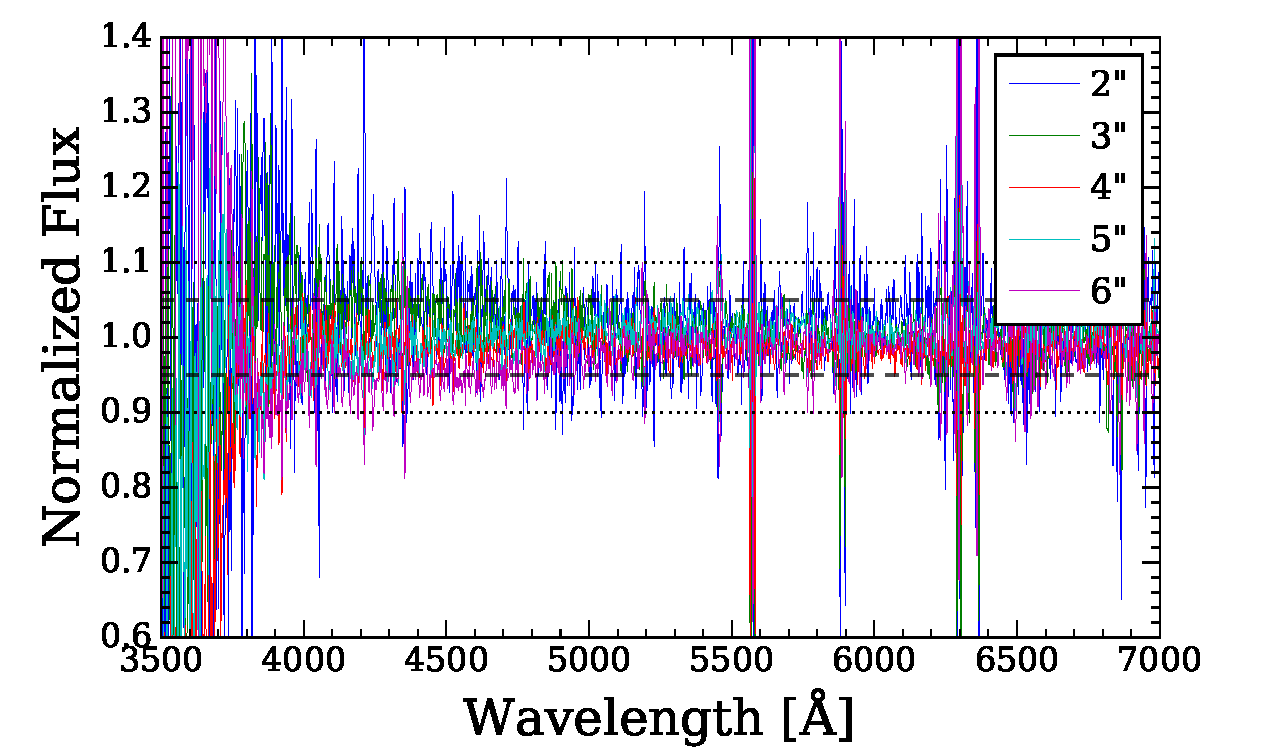
\includegraphics[width=\columnwidth]{891_1/figs/flux_cal_test.pdf}
  \caption[Comparison of flux calibration across multiple fiber
    sizes]{ \label{891_1:fig:sky_flux_comp}\fixspacing Flux
    calibration test for all fiber sizes when using standard star data
    from only 5.62'' fibers. Data are taken from a single galaxy
    exposure reduced through flux calibration, but not
    sky-subtracted. Each line represents the average of all 4 sky
    fibers for a given fiber size and all lines are normalized by the
    mean of all sky fibers. The dashed and dotted lines show
    deviations at the 5\% and 10\% level, respectively. All fiber
    sizes show an absolute flux calibration consistent within 5\% for
    wavelengths $>$ \val{4000}{\AA}. At \val{4000}{\AA} the 2 arcsec
    and 3 arcsec fibers deviate by up to 20\%.}
\end{figure}

\subsection{Flux Calibration}
\label{891_1:sec:flux_cal}

%% {\bf [TO DO: There is basic argument that we need to make for why we
%%     think application of the flux cal from the large fibers to all
%%     fibers is valid. This consists of a combination of the fact that
%%     all of the fiber is of the same material. However, beause it is
%%     not necessarily from the same draw, there could be
%%     variations. That is where information from lab measurements in the
%%     \GP instrument description section would be useful.]} 

As discussed in \S\ref{891_1:sec:cal_data} atmospheric refraction limited
our standard star observations to only the 5.62'' fibers. On each
night the same two standard stars were observed in multiple 5.62''
fibers and a flux calibration was computed using the ONEDSPEC
package. Time constraints in our observing program limited the range
of airmasses available for standard star observations and for this
reason we could not compute an extinction curve for our data. We
instead used the KPNO extinction curve provided in
ONEDSTDS\footnote{http://stsdas.stsci.edu/cgi-bin/gethelp.cgi?onedstds}.

\begin{figure}
  \centering
  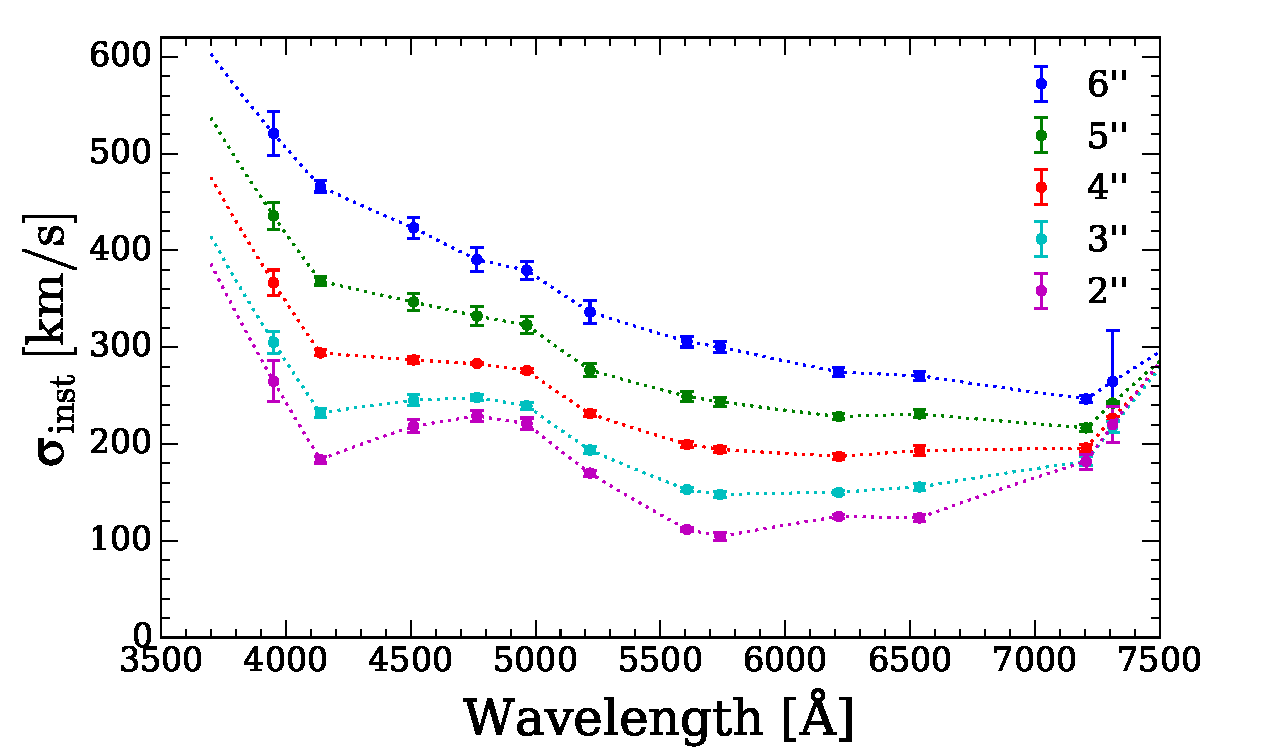
\includegraphics[width=\columnwidth]{891_1/figs/disp_paper.pdf}

  \caption[Variation of instrumental resolution in \GP
  fibers]{\label{891_1:fig:dispfunc}\fixspacing Instrumental resolution as
    measured from CuAr arc-lamps (see text) are plotted as points; the
    interpolated and extrapolated dispersion functions used in
    spectral modeling is shown by the dotted lines.}
\end{figure}

To zeroth order we expect the spectral response of all the \GP fibers
to be the same because they are made of the same material and are all
from the same foundry run \citep{Wood12}. In reality the \GP fibers
come from different draws, were handled differently during
construction, and have different degrees of termination quality.
Consequently, there are throughput variations not only between fiber
sizes, but also within fiber sizes, as illustrated in Figure
\ref{GPtesting:fig:TL_FRD}.  Throughput characteristics vary across the \GP
array. In particular, the total throughput and focal ratio degradation
are worse for the smallest fibers. The throughput variations are
expected to relatively grey (wavelength independent), but since there
are variations in FRD, this can lead to different, wave-length
dependent losses within the spectrograph. Since the flat-field screen
uniformly illuminates the array, the flat-fielding process should
remove all of these relative variations.

To assess the effects of using flux standards taken in a single fiber
size to calibrate the entire \GP IFU we compared flux calibrated sky
spectra for all fiber sizes. The data came from a single exposure of
P3 (see Figure \ref{891_1:fig:pointings}) where none of they sky spectra
appeared to be outliers due to source contamination from foreground
stars or background galaxies.  All sky fibers were flux calibrated
using data from the 5.62'' fibers, and then the 4 sky fibers of each
size were averaged together. Figure \ref{891_1:fig:sky_flux_comp} shows the
average spectrum for each fiber size, normalized to the mean of
\emph{all} sky fibers. At wavelengths greater than \val{4000}{\AA} the
sky spectra are consistent between fiber sizes to within 5\%. Below
\val{4000}{\AA} the flux calibration varies by up to $\asim$20\% due
to low signal to noise at these wavelengths.

%% {\bf Here's what MAB doesn't understand: (a) why do the
%%   strong sky lines, like OI at 5563 or so, show such large variations?
%%   (b) you say the flux cal varies a lot below 4000A due to low SNR in
%%   the smallest fibers yet the magenta curve for the 6'' fibers seems
%%   as aberrant as any.}

To account for night-to-night offsets in extinction (caused by, e.g.,
high cirrus clouds) we scaled each individual exposure so that all
exposures in a particular pointing have the same average flux in the
region $\val{4500}{\AA} \leq \lambda \leq \val{5500}{\AA}$. Within a
single night this scaling was always less than \asim 3\%, but between
nights it could vary by a factor of up to 2 in cases where a night had
poor observation conditions (high humidity, persistent clouds,
etc.). The final spectra for each pointing are an average of
individual exposures weighted by the square of the inverse of their
deviation from the mean pointing flux in the range $\val{4500}{\AA}
\leq \lambda \leq \val{5500}{\AA}$.

\subsection{Instrumental Line Profile}
\label{891_1:sec:GPak_dispersion}

The optical distortions of the WIYN Bench Spectrograph result in an
instrumental line profile that varies with wavelength and field
location along the fiber slit for a fiber of a given size. The
delivered line profile in the spectral dimension (the instrumental
dispersion) is a convolution of this distortion with the
anamorphically demagnified fiber image. Consequently the different
fiber sizes in \GP cause the spectral line profile to be a different
function of wavelength for each fiber size. We refer to this value as
$\sigma_{\rm inst}$, reported in units of km/s.

To account for the variations in $\sigma_{\rm inst}$ in our later
fitting of model spectral energy distributions, we first measured the
width of arc-lamp emission lines across our entire wavelength range
for all fibers. Widths for each arc line were measured for every
fiber, and then averaged for all fibers of the same size, weighted by
poisson noise in each fiber. Arc lines with low signal-to-noise were
combined together in groups over narrow wavelength ranges to improve
the signal and assigned a new wavelength weighted by the
signal-to-noise of the component lines. This was particularly
important in the far blue where the lines were few and often
weak.

These data were interpolated to create dispersion functions,
$\sigma_{{\rm inst},i}(\lambda)$, for each fiber size, $i$. Past the
blue and red ends of the region covered by arc lines
(\val{4130}{\AA}$<\lambda <$ \val{7300}{\AA}) the dispersion functions
are extended with linear extrapolation. The line-width data and
resulting instrumental dispersion functions can be found in Figure
\ref{891_1:fig:dispfunc}. Note the hat-shaped profile seen for the smallest
fibers, characteristic of the typical compromise focus value chosen
for the all refractive Bench Spectrograph system. For larger fiber
sizes the resolution is dominated by the geometric fiber diameter and
the changes in the grating dispersion with wavelength.


